\documentclass[10pt]{article}
\usepackage[T1]{fontenc}\usepackage{lmodern,amsmath,amssymb,graphicx,hyperref}
\usepackage[margin=.76in]{geometry}
\setlength{\parindent}{0pt}\setlength{\parskip}{7pt}
\begin{document}
\begin{center}{\Large Actual shared-profile first-moment obstruction}\\[4pt]
Local continuation --- 15 November 2026\end{center}
\textbf{Actual formula.} Let $i<u\le a$, use one arbitrary common natural
multiplicity profile $m$, node $-2^i$, truncation $k=2$, moment $b=1$ and
matching residue/classPort column. Set
\[
 c_j=\frac{2^u}{2^j},\qquad B(m)=\sum_{j<u}m_jc_j.
\]
The actual right factor satisfies
\[
 [Z^1]R_{i,(r,1),r}=\frac{c_i-B(m)}2.
\]
This is derived from the actual factor definitions, not a supplied
coefficient witness. It holds for every residue and every common $m$;
no global feasibility or favorable multiplicity premise is inserted
[pcc:unverified].

\textbf{Instance chain.} Mapping the actual denominator by the constant
coefficient in $Z$ gives
\[
 D_i(H,0)=(1-c_iH)\prod_{j<u}(1+c_jH)^{m_j}.
\]
The new generic owning-library law, assembled from Mathlib derivative,
product, power and evaluation rules, gives
$[H^1]D_i(H,0)=-c_i+B(m)$. The actual normalized numerator already has
constant coefficient zero and first coefficient one. At $k=2$, the finite
geometric sum is $2-D_i$. The actual moment normalization divides its
$H^1$ coefficient by two, yielding the displayed right-factor formula
[pcc:unverified].

\textbf{Two-node control.} When $u\ge2$, the two highest retained nodes
have $c_{u-2}=4$ and $c_{u-1}=2$. Consequently
\[
 [Z^1]R_{u-2,(r,1),r}-[Z^1]R_{u-1,(r,1),r}=1.
\]
Both coefficients therefore cannot have valuation at least one. The source
uses the existing valuation-bound addition and negation laws: the difference
of two such coefficients would have the same bound, contradicting
$v_2(1)=0$ [pcc:unverified].

\textbf{Scoped consequence.} No common $m$ makes every retained matching
first-moment right polynomial Content1, or Content2, for this exact
$k=2$ factorization. Thus uniform odd-factor rescaling at every node cannot
be obtained merely by choosing a different multiplicity profile here.
This is stronger than rejecting the earlier sufficient mod-four residue
contract, because it uses the actual coefficients [pcc:unverified].

\textbf{Boundary.} This is a right-factor statement. At $a=u$, higher left
moments vanish. A weighted-active conclusion requires $a>u$ and a separate
nonzero left witness. Neither different factorizations, variable truncation
schedules, nonuniform gains nor general algorithms are excluded
[pcc:unverified].
\newpage
\begin{center}{\Large Validation and the nonuniform continuation}\end{center}
\begin{center}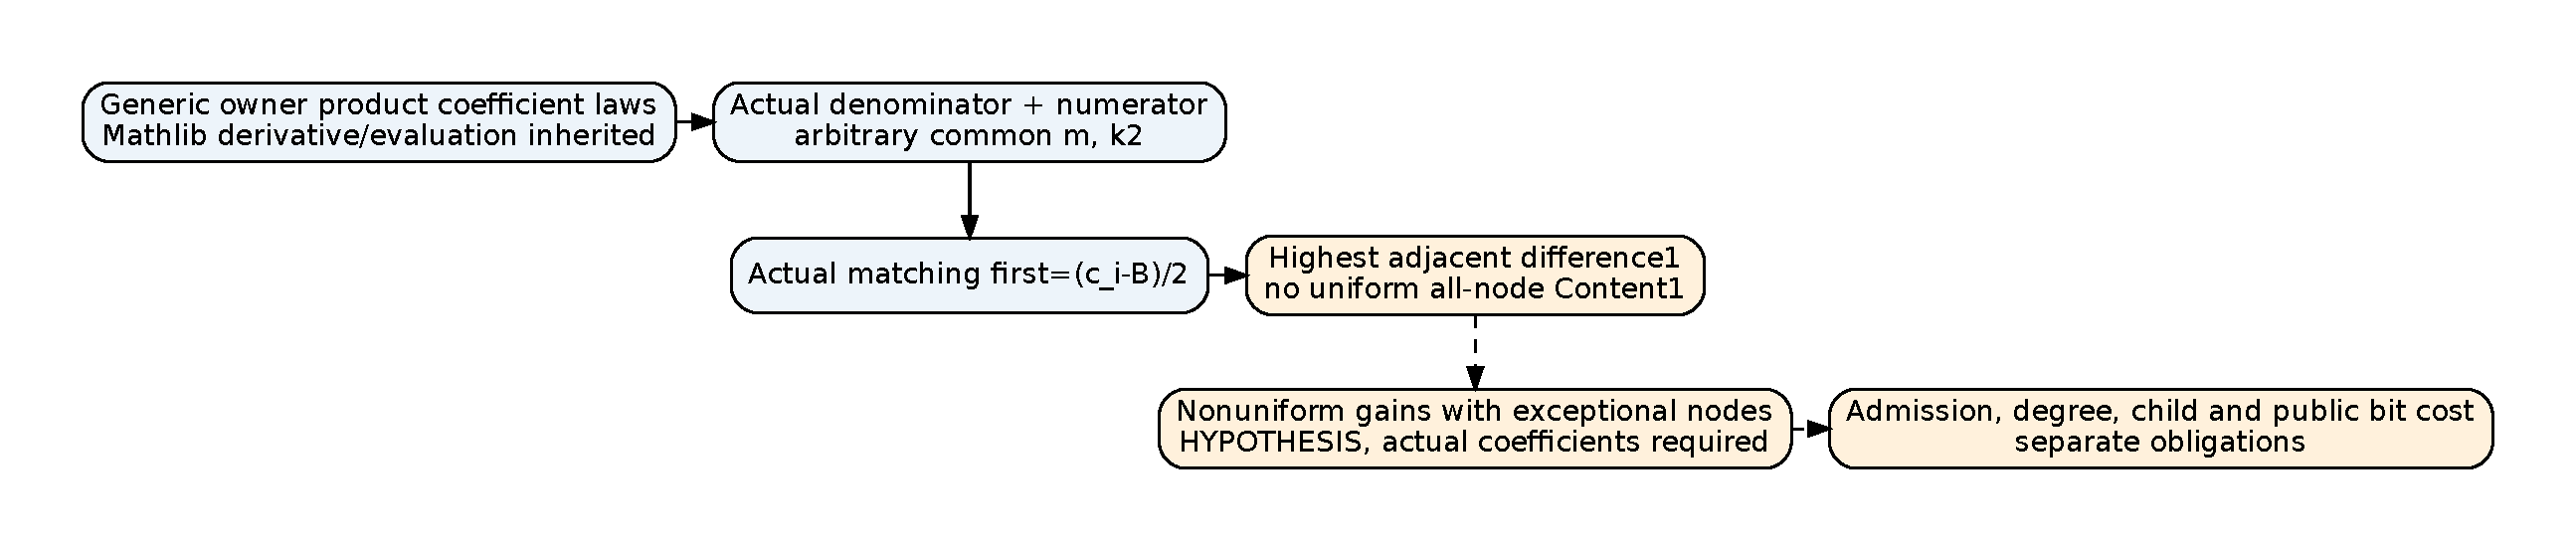
\includegraphics[width=\linewidth,height=2.5in,keepaspectratio]{shared-first-moment-dependencies-001.pdf}\end{center}
\textbf{Accepted evidence.} Local100 has435 statements including parent432,
three new;101 has439 including435, four new. Both exit zero without warnings
or sorryAx. Receipts050 and051 bind the exact source, raw output and exit.
Central printed dependencies are standard. Failed098 and099 are retained
[pcc:unverified].

\textbf{Owning-library law.} Isolated CryptoLean commit93b303be contains
coefficient0 and coefficient1 laws for finite products of linear powers
over any commutative semiring. Existing Mathlib rules are reused as stated;
no generic induction is copied into the study. The affected target build
has no warnings, and the pinned module axiom auditor reports two theorems,
zero failing and zero trusted. Receipt049 preserves accepted and failed
owner source versions and raw logs. Consumer manifests and old dependency
pins are unchanged; the experimental import overlay is explicit. This is
not a full repository gate, fresh replay or signed verdict
[pcc:unverified].

\textbf{New hypothesis.} Keep one common profile $m_j=4n_j$. Test full
odd-factor gains two bits at lower nodes, one at the penultimate node and
no extra gain at the highest node. Those bounds remain unproved. The
highest-node exception must stay in the cost model. The generic fourth-power
probe is standard arithmetic; its actual instance must be over the existing
two-integral rational subring, not merely $\mathbb Q$, where divisibility by
four gives no valuation information [pcc:unverified].

\textbf{Required cost bridge.} Construct $n$ from an actually admitted
schedule, derive the multiplicity, mass and degree scaling, retain every
$2^uk$ label and charge exceptional nodes, creation precision, child entries
and all preparation and bit costs. A finite local content gain alone gives
no asymptotic exponent conclusion. Original elliptic relation, public
finder and scalar recovery remain separate interfaces
[pcc:unverified].

\textbf{Preservation.} All earlier sources, evidence, claims and report pins
remain exact. The owned module's canonical archival source copy is a derived
payload hydrated byte-for-byte from tracked source003 text; no receipt hash
changes and no binary/cache is tracked. Remote protected ledger publication
remains withheld; independent local mathematics continues. No native,
timing, scaling, paid/cloud or attack experiment was run.
\end{document}
